\documentclass{acm_proc_article-sp}
\makeatletter
\def\@copyrightspace{\relax}
\makeatother

\usepackage{graphicx}

\begin{document}

% 1. Report title, authors, and support cast (Lab assistant and course instructors). For each person, give name and contact information (email).
\title{GaussianCloud}
\subtitle{A cloud-based image blurring application}

\numberofauthors{5}
\author{
\alignauthor
R.M. de Lange\\
		\affaddr{1534068}\\
		\email{\{r.m.delange,}
\alignauthor
M. Voinea\\
		\affaddr{4317602}\\
		\email{m.voinea\}@student.tudelft.nl}
\and
\alignauthor
D.H.J. Epema\\
		\affaddr{Course Instructor}\\
		\email{\{d.h.j.epema,}
\alignauthor
A. Iosup\\
		\affaddr{Course Instructor}\\
		\email{a.iosup,}
\alignauthor
B.I. Ghit\\
		\affaddr{Lab Assistant}\\
		\email{b.i.ghit\}@tudelft.nl}
}

\maketitle

% 2. Abstract: a description of the problem, system description, analysis overview, and one main result. Size: one paragraph with at most 150 words.
\begin{abstract}
\end{abstract}

% 3. Introduction (recommended size, including points 1 and 2: 1 page): describe the
% problem, the existing systems and/or tools (related work), the system you are about to
% implement, and the structure of the remainder of the article; use one short paragraph
% for each.
\section{Introduction}
WantCloud BV is an organisation with a large workload in blurring images.
One of the business processes in WantCloud requires large images to be blurred using a Gaussian blur.
This process is compute intensive, as Gaussian functions require complex calculations as well as reading and writing a large amount of data.

Currently, WantCloud has a single server running all of these tasks.
This machine is experiencing heavy peak loads and sits idle for the rest of the day
Therefore, WantCloud wants to explore the option to employ the cloud to be able to scale up and down as needed.

This report will discuss the details of an exploration towards using Amazon EC2\footnote{http://aws.amazon.com/ec2/} as a solution to WantClouds needs.
The image processing system will be implemented on a dynamically scalable cluster of compute nodes.
This implementation is made available open-source through GitHub\footnote{https://github.com/mickdelange/cclab}.
The performance, overhead, and scalability will be tested to compare to the current set-up using one machine.

This paper will first give an insight in the application and its requirements in Section \ref{sec_bg}.
After this the design of the cloud system will be discussed in Section \ref{sec_system}, giving an insight in the implementation.
The designed system will be evaluated in Section \ref{sec_eval}.
The results in the evaluation will be discussed in Section \ref{sec_discussion} and conclusions will be presented in Section \ref{sec_conclusion}.

% 4. Background on Application (recommended size: 0.5 pages):
% describe the application (1 paragraph) and its requirements (1-3 paragraphs, summarized in a table if needed).
\section{Background}
\label{sec_bg}
The application that this report describes handles image files and adds Gaussian Blur to these images.
Image files can be uploaded, which will then be processed and the results will be returned to the user.
The application uses the Amazon Compute Cloud to process the images in a reliable and scalable way.
This means that the number of used nodes -and therefore the resulting cost- is kept to a minimum, whilst providing better performance than WantCloud currently has.
More specifically, the application has to deal with the following requirements.

\subsection{Elasticity}
The application must scale the active nodes up and down depending on the workload.
This means that unused nodes should be released as they are no longer needed, and new nodes should be leased as soon as the workload increases.
This requirement should result in lower cost for maintaining nodes, while handling peak loads faster.

\subsection{Automation}
The application should handle its own scheduling automatically.
This means that tasks are assigned to available nodes, new nodes are started when needed, and unused nodes are release without human input.

\subsection{Fault tolerance}
Furthermore, the application must be reliable, or fault tolerant.
This means that any problems that occur should be dealt with by the system itself.
Nodes that crash, tasks that break or other problems that occur should be dealt with by the system itself, again without human input.

% 5. System Design (recommended size: 1.5 pages)
% a. Resource Management Architecture: describe the design of your system,
% including the inter-operation of the provisioning, allocation, reliability, and
% monitoring components (which correspond to the homonym features required
% by the WantCloud CTO).
% b. System Policies: describe the policies your system uses and supports. The latter
% may remain not implemented throughout your coursework, as long as you can
% explain how they can be supported in the future.
% c. (Optional, for bonus points, see Section F) Additional System Features:
% describe each additional feature of your system, one sub-section per feature.
\section{System Design}
\label{sec_system}
The system design is aimed at providing a simple platform to support the work that WantCloud wants to perform.
It is intended as a proof of concept, rather than a production ready solution.
With this in mind, the main design decision were made to comply with the requirements discussed in Section \ref{sec_bg}.
In this section the main aspects of the system design will be discussed: the architecture, resource management, and policies.

\subsection{Architecture Overview}
The architecture of this solution is kept very simple, it consists of Master and Worker nodes.
These nodes communicate to notify each other of new tasks and finished tasks.
% TODO: Mick create a visualisation of the architecture.

\subsubsection{Master}
The Master node manages the process, it handles the scheduling and assigns tasks to Worker nodes.
As a new task comes in to the Master node, it is added to its main queue and assigned to the first available Worker.
If no Worker nodes are available, a new node is started to handle the workload.
The Master is also responsible for keeping track of each Worker's queue.
Worker nodes do not maintain a queue themselves, but are rather assigned one task at a time.

\subsubsection{Worker}
Worker nodes perform the actual work.
These nodes receive tasks from the Master node, process them, and reply to the Master whenever a task is finished.
Worker nodes are not aware of the length of their queue, the Master node keeps track of this information.
This design choice was made to keep the Worker nodes as simple as possible and also allow for easy fault correction in case a Worker node crashes.

\subsubsection{Communication}
% TODO: Maria describe the communication between nodes

\subsection{Resource Management Architecture}
The resources used in this application are a number of EC2 instances.
For testing purposes the free \texttt{t2.micro} instances where used with an Ubuntu operating system.
Here we will discuss how the requirements set in Section \ref{sec_bg} can be satisfied by the designed architecture.

\subsubsection{Elasticity}

\subsubsection{Automation}

\subsubsection{Fault Tolerance}

\subsection{System Policies}

\subsubsection{Scheduling}

\subsubsection{Redundancy}

\subsubsection{Extensions}

% 6. Experimental Results (recommended size: 1.5 pages)
% a. Experimental setup: describe the working environments (DAS, Amazon EC2,
% etc.), the general workload and monitoring tools and libraries, other tools and
% libraries you have used to implement and deploy your system, other tools and
% libraries used to conduct your experiments.
% b. Experiments: describe the experiments you have conducted to analyze each
% system feature, then analyze them; use one sub-section per experiment. For
% each experiment, describe the workload, present the operation of the system,
% and analyze the results. In the analysis, report:
% i. Charged-time = time that would have been charged using the
% Amazon EC2 timing approach (1-hour increments)
% ii. Charged-cost = cost that would have been charged using the
% Amazon EC2 charging approach, assuming 10 Euro-cents/charged hour
% iii. Service metrics of the experiment, such as runtime and response time of
% the service, etc.
% iv. (optional) Usage metrics of the experiment, such as per-VM and overall
% system usage and activity.
\section{Evaluation}
\label{sec_eval}

\subsection{Setup}

\subsection{Test files}

\subsection{Experiments}

\subsubsection{Scheduler}
\begin{figure}[]
	\centering
	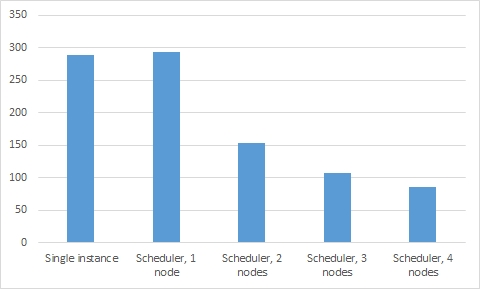
\includegraphics[width=0.5\textwidth]{images/diagram_total_processing.jpg}
	\caption{Processing time comparison for 5 types of setups. Time in seconds.}
	\label{fig:diagram_total_processing}
\end{figure}


% 7. Discussion (recommended size: 1 page): summarize the main findings of your work
% and discuss the tradeoffs inherent in the design of cloud-computing-based applications.
% Should the WantCloud CTO use IaaS-based clouds? Among others, use extrapolation
% on the results, as reported in Section 6.b of the report, to discuss the charged time and
% charged cost reported in section for 100,000/1,000,000/10,000,000 users and for 1
% day/1 month/1 year.
\section{Discussion}
\label{sec_discussion}

% 8. Conclusion
\section{Conclusion}
\label{sec_conclusion}

\bibliography{references}{}
\bibliographystyle{plain}

\appendix
% 9. Appendix A: Time sheets (see Section E)
\section{Time sheet}

The following table documents the time spent working on the assignment.

\begin{tabular}{ | l | r | }
	\hline
	Part & Time (hrs) \\ \hline \hline
	% the  = total amount of time spent in completing WantOne CTO’s assignment (the large exercise).
	\texttt{total-time} & 50\\ \hline
	% the think-time = total amount of time spent in thinking about how to solve WantOne CTO’s assignment (the large exercise).
	\texttt{think-time} & 8\\ \hline
	% the dev-time = total amount of time spent in developing the code needed to solve WantOne CTO’s assignment (the large exercise).
	\texttt{dev-time} & 40\\ \hline
	% the xp-time = total amount of time spent in experiments for WantOne CTO’s assignment (the large exercise).
	\texttt{xp-time} & 0\\ \hline
	% the analysis-time = total amount of time spent in analyzing the results of the experiments for WantOne CTO’s assignment (the large exercise).
	\texttt{analysis-time} & 0\\ \hline
	% the write-time = total amount of time spent in writing this report
	\texttt{write-time} & 2\\ \hline
	% the wasted-time = total amount of time spent in activities related to WantOne CTO’s assignment (the large exercise), but which cannot be charged as think-time, dev-time, xp-time, analysis-time, or write-time
	\texttt{wasted-time} & 0\\ \hline
\end{tabular}

\end{document}